
\chapter{Transformadores y Estad\'istica Bayesiana}

\noindent En esta tesina se propone un plan de inventario de transformadores de instrumento,
 desde un enfoque Bayesiano. Para lograr esta meta, se necesita primero conocer aspectos exploratorios sobre el comportamiento del tiempo de  vida de los transformadores.  
 
 
\noindent Para empezar el estudio que nos conduzca al plan de inventario o almacenamiento, tenemos que realizar inferencia 
sobre los datos e informaci\'on disponible.\\[0.1cm] 
En este cap\'itulo se hace el an\'alisis de los datos,  proponiendo 
una distribuci\'on a priori, para combinarla con la funci\'on de verosimilitud y tener la distribuci\'on 
posterior, para conseguir conclusiones acerca del comportamiento de los tiempos de vida de
los transformadores.


\begin{table}[h!]\small
\begin{center}
\caption {\bf Tiempos de vida de transformadores de corriente, $t_i$ (meses), $e_i=1$ indica un dato censurado, $e_i=0$ es un dato no censurado.\label{uno}}
\begin{tabular}{ccc|ccc|ccc|ccc}
\toprule[0.6mm]
$i$	&	$t_i$	&	$t_i$	&	$i$	&	$t_i$	&$e_i$	&	$i$	&	$t_i$	&	$e_i$	&	$i$	&	$t_i$	&	$e_i$	\\
\toprule[0.6mm]
1	&	8	&	1	&	36	&	107	&	0	&	106	&	272	&	1	&	141	&	308	&	0	\\
2	&	8	&	1	&	37	&	116	&	1	&	107	&	272	&	1	&	142	&	308	&	0	\\
3	&	8	&	1	&	38	&	119	&	0	&	108	&	272	&	1	&	143	&	308	&	1	\\
4	&	8	&	1	&	39	&	119	&	0	&	109	&	272	&	1	&	144	&	308	&	1	\\
5	&	8	&	1	&	40	&	139	&	0	&	110	&	272	&	1	&	145	&	308	&	1	\\
6	&	20	&	1	&	41	&	140	&	0	&	111	&	274	&	0	&	146	&	308	&	1	\\
7	&	20	&	1	&	42	&	144	&	0	&	112	&	274	&	0	&	147	&	308	&	1	\\
8	&	20	&	1	&	43	&	146	&	0	&	113	&	274	&	0	&	148	&	308	&	1	\\
9	&	20	&	1	&	44	&	146	&	0	&	114	&	275	&	0	&	149	&	308	&	1	\\
10	&	32	&	1	&	45	&	152	&	1	&	115	&	275	&	0	&	150	&	308	&	1	\\
11	&	32	&	1	&	46	&	159	&	0	&	116	&	275	&	0	&	151	&	308	&	1	\\
12	&	32	&	1	&	47	&	159	&	0	&	117	&	276	&	0	&	152	&	308	&	1	\\
13	&	32	&	1	&	48	&	159	&	0	&	118	&	281	&	0	&	153	&	308	&	1	\\
14	&	32	&	1	&	49	&	160	&	0	&	119	&	281	&	0	&	154	&	308	&	1	\\
15	&	32	&	1	&	50	&	161	&	0	&	120	&	284	&	0	&	155	&	308	&	1	\\
16	&	32	&	1	&	51	&	164	&	1	&	121	&	284	&	0	&	156	&	308	&	1	\\
17	&	56	&	1	&	52	&	167	&	0	&	122	&	284	&	0	&	157	&	308	&	1	\\
18	&	80	&	1	&	53	&	172	&	0	&	123	&	284	&	0	&	158	&	308	&	1	\\
19	&	80	&	1	&	54	&	172	&	0	&	124	&	286	&	0	&	159	&	308	&	1	\\
20	&	80	&	1	&	55	&	176	&	1	&	125	&	286	&	0	&	160	&	308	&	1	\\
21	&	80	&	1	&	56	&	183	&	0	&	126	&	286	&	0	&	161	&	308	&	1	\\
22	&	80	&	1	&	57	&	188	&	1	&	127	&	287	&	0	&	162	&	308	&	1	\\
23	&	80	&	1	&	58	&	203	&	0	&	128	&	288	&	0	&	163	&	308	&	1	\\
24	&	80	&	1	&	59	&	205	&	0	&	129	&	288	&	0	&	164	&	308	&	1	\\
25	&	80	&	1	&	60	&	214	&	0	&	130	&	288	&	0	&	165	&	308	&	1	\\
26	&	80	&	1	&	61	&	214	&	0	&	131	&	288	&	0	&	166	&	308	&	1	\\
27	&	80	&	1	&	62	&	215	&	0	&	132	&	296	&	1	&	167	&	308	&	1	\\
28	&	80	&	1	&	63	&	216	&	0	&	133	&	296	&	1	&	168	&	308	&	1	\\
29	&	80	&	1	&	64	&	216	&	0	&	134	&	296	&	1	&	169	&	308	&	1	\\
30	&	80	&	1	&	65	&	216	&	0	&	135	&	296	&	1	&	170	&	308	&	1	\\
31	&	80	&	1	&	66	&	218	&	0	&	136	&	298	&	0	&	171	&	308	&	1	\\
32	&	80	&	1	&	67	&	218	&	0	&	137	&	299	&	0	&	172	&	308	&	1	\\
33	&	94	&	0	&	68	&	218	&	0	&	138	&	300	&	0	&	173	&	308	&	1	\\
34	&	94	&	0	&	69	&	225	&	0	&	139	&	308	&	0	&		&		&		\\
35	&	94	&	0	&	70	&	225	&	0	&	140	&	308	&	0	&		&		&		\\
\bottomrule[0.6mm]
\end{tabular}
\end{center}
\end{table}


\section{Distribuci\'on Apriori}
\noindent Los elementos disponibles dentro del estudio, 
es una base de datos de transformadores de instrumento de corriente en las sub\'areas de  
Coatzacoalcos y Temascal. Se disponen de sus tiempos de vida  a lo largo de 26 a\~nos hasta el 2006, con datos censurados y no 
censurados. 

\noindent Los datos se muestran en la Tabla \ref{uno}, representados de la siguiente manera, 
$(\underline{t},\underline{e})=\{t_i,e_i\}^n_{i=1}$, donde $e_i=1$ indica que 
el transformador $i$ aun sigui\'o en 
operaci\'on al final de 2006, lo que implica que  es un dato censurado por la derecha. Mientras que $e_i=0$, se refiere a un valor no censurado. De estudios 
anteriores realizados por el CIMAT, los tiempos de vida son modelados adecuadamente 
por medio de una 
distribuci\'on Weibull. La funci\'on de Verosimilitud bajo 
este modelo se expresa 
de la siguiente manera:
\begin{eqnarray}\label{tiempos}
f(\underline{t}|\underline{e},\beta,\eta)&=& \prod_{e_i=0}\frac{\beta}{\eta}\left(\frac{t_i}{\eta}\right)^{\beta-1}\exp \left\{-\left(\frac{t_i}{\eta}\right)^{\beta}\right\}\prod_{e_i=1}\exp\left\{-\left(\frac{t_i}{\eta}\right)^{\beta}\right\}.
\end{eqnarray}

\noindent Para iniciar la inferencia de los datos disponibles, necesitamos proponer una distribuci\'on a priori que refleje el conocimiento que se tiene acerca del fen\'omeno a modelar. Elegimos como modelo para los par\'ametros  $\beta$ y $\eta$ distribuciones gammas, con la siguiente notaci\'on:
\begin{eqnarray}\label{beta}
\beta\sim Ga(a_1,b_1)
\end{eqnarray}
 y 
  \begin{eqnarray}\label{eta}
 \eta\sim Ga(a_2,b_2). 
 \end{eqnarray}
 
\noindent La raz\'on por la cual elegir  distribuciones Gammas para las a  prioris  es su flexibilidad, pueden obtenerse formas sesgadas a la derecha, izquierda o centradas. Cabe mencionar que la elecci\'on de una distribuci\'on a priori  espec\'ifica, solo se debe de interpretar como un medio o instrumento  que nos ayudar\'a a modelar la informaci\'on disponible.\\[0.2cm]
 \noindent Una vez elegidos los instrumentos de modelaci\'on, es de inter\'es establecer los par\'ametros para las a prioris, estos se fijar\'an con la ayuda de dos elementos:
\begin{itemize}
\item  La distribuci\'on predictiva a priori.
\item  El comportamiento de la funci\'on de riesgo de los transformadores.
\end{itemize}

\begin{figure}
\begin{center}
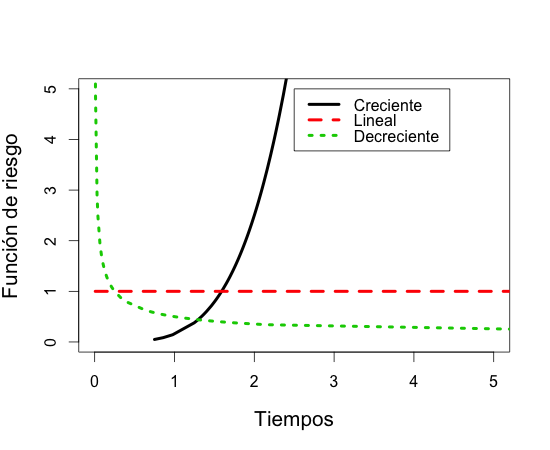
\includegraphics[scale=0.4]{r1.png}
\end{center}
\vspace{-1 cm}\caption{\bf Posibles funciones de riesgo para la distribuci\'on predictiva a priori.}\label{trestt}
\end{figure}


\noindent Primero hablaremos acerca de la funci\'on de riesgo.  Esta funci\'on describe el desgaste de los transformadores a lo largo del tiempo. Al empezar su funcionamiento, el riesgo a fallar es peque\~no y conforme pasa el tiempo, debido al uso, el ambiente y otros factores, el riesgo aumenta paulatinamente. La determinaci\'on o modelaci\'on de las distribuciones a priori tienen como misi\'on descartar entornos improbables de los fen\'omenos que modelan. En la Figura  \ref{trestt} se observan tres trayectorias posibles de riesgo.
Si la vida de los transformadores tiene una funci\'on de riesgo decreciente, indica  que al momento de iniciar su vida \'util, el riesgo a fallar es alto y conforme pasa el tiempo, se reduce.  Sin embargo existen factores como la humedad que no permiten que el riesgo de falla de un transformador disminuya, sino al contrario.\\[0.1cm]
\noindent  Por otra parte si la funci\'on de riesgo es constante, se concluir\'ia que los transformadores no se degradan a trav\'es del tiempo. Lo que no ocurre dadas las condiciones de uso.
\noindent As\'i la funci\'on de riesgo adecuada, es aquella que indique que en los primeros a\~nos de vida su riesgo es peque\~no y a lo largo del tiempo este riesgo aumenta. Una funci\'on de riesgo creciente es la m\'as razonable de acuerdo al funcionamiento de los transformadores. 

\noindent Por lo tanto la distribuci\'on a priori propuesta debe tener una funci\'on de riesgo creciente, esto es el par\'ametro $\beta$ tiene que ser mayor que $1$. \\[0.1cm]
\noindent
El siguiente paso, es observar el comportamiento de la distribuci\'on predictiva a priori. Previamente se mencion\'o la manera en la cual se obtiene la distribuci\'on predictiva posterior, sin embargo no se coment\'o nada al respecto de la {\bf distribuci\'on predictiva a priori}.  Al momento de asignar una distribuci\'on de probabilidad a los par\'ametros ($\beta$, $\eta$), estos no tienen interpretaci\'on cuantificable por experiencias. No es posible conocer expl\'icitamente sus valores por observaciones previas, solo tenemos conocimiento del fen\'omeno en general. Si se sabe la manera a priori del comportamiento del tiempo de vida de los transformadores entonces se tiene conocimiento de la distribuci\'on predictiva a priori. Esta distribuci\'on esta dada por:

 $$f(t)=\int_{\beta,\eta}f(t|\beta,\eta)  f(\beta,\eta)d\beta d \eta,$$
 
 \noindent donde  $f(\beta,\eta)$ es la distribuci\'on conjunta a priori de $\beta$ y $\eta$.
\noindent Por experiencia podemos conocer ciertas caracter\'isticas del tiempo de vida de los transformadores y  tener informaci\'on previa de  $f(t)$. Esta informaci\'on determina un rango de valores para $\beta$ y $\eta$. La manera m\'as com\'un de establecer la distribuci\'on  a priori predictiva es empleando dos cuantiles. Como describiremos en los siguientes p\'arrafos.\\[0.1cm]


%\\[0.2cm]
\begin{figure}
\begin{center}
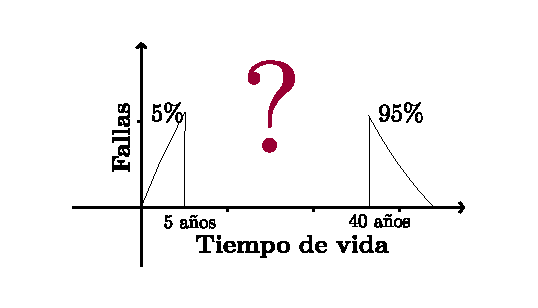
\includegraphics[scale=1]{apriori1.pdf}
\end{center}
\vspace{-1.5 cm}\caption{\bf Distribuci\'on predictiva a priori a modelar.}\label{dos}
\end{figure}

\noindent  Suponiendo que el $5\%$ de los transformadores fallan en los primeros 5 a\~nos (80 meses) y  que el $95\%$ de ellos ya fallaron a los $40$ a\~nos (480 meses) o antes, y 
si adem\'as $$T\sim \text{Weibull}(\eta^{*},\beta^{*})$$ 


\noindent es la variable aleatoria a priori que modela el tiempo de vida de los transformadores. La Figura \ref{dos} muestra la distribuci\'on a priori predictiva, con los cuantiles fijados en los extremos. Sin embargo el centro de la distribuci\'on debe ser modelada.\\[0.1cm]
\noindent La informaci\'on de los cuantiles se representa por:
$$P(T\leq 80)=0.05$$
y 
$$P(T\leq 480)=0.95.$$

\noindent Con esta informaci\'on es posible conocer  $\eta^{*}$ y  $\beta^{*}$  de la siguiente forma, se sabe que para una variable aleatoria Weibull
\begin{eqnarray*}
P(T\leq t) &=& 1-\exp\left\{-\left(\frac{t}{\eta}\right)^{\beta}\right\}
\end{eqnarray*}

Por lo tanto debemos resolver
\begin{eqnarray*}
0.05 &=& 1-\exp\left\{-\left(\frac{t}{\eta^{*}}\right)^{\beta^{*}}\right\}\\
0.95 &=& 1-\exp\left\{-\left(\frac{t}{\eta^{*}}\right)^{\beta^{*}}\right\}\\
\end{eqnarray*}

Resolviendo el sistema se llega a que

\begin{eqnarray*}
\beta^{*}&=& 1.955\\
\eta^{*}&=& 273.8
\end{eqnarray*}

\noindent Los par\'ametros encontrados describen el comportamiento a priori del tiempo de vida, no de los par\'ametros $\beta$  y $\eta$. Con ayuda de estos datos se pueden obtener los par\'ametros $a_1, b_1, a_2$ y $b_2$, que como lo mencionamos al inicio de la secci\'on son los par\'ametros, para las distribuciones Gammas de  $\beta$ y $\eta$ respectivamente, notando lo siguiente:

\begin{enumerate}
\item[{\bf 1.-} ]
\noindent  Como $\beta^{*}= 1.955$, quiere decir que los valores que produzca la distribuci\'on Gamma con par\'ametros $a_1$ y $b_1$ oscilaran alrededor de estos valores. Similarmente como $\eta^{*}= 273.8$ significa que los valores que tome la distribuci\'on $Ga(a_2,b_2)$ estar\'an alrededor de 273.8 aproximadamente.
\item[{\bf 2.-} ]
\noindent De manera general  la funci\'on de densidad de una variable aleatoria Gamma con par\'ametros $a$ y $s$, representada como $Ga(a,s)$ es

$$f(x)=\frac{1}{s^a\Gamma(a)}x^{a-1}\exp\left\{\frac{x}{s}\right\}$$
y su valor esperado esta dado por:
\begin{eqnarray*}
E(X)&=& as.
\end{eqnarray*}

\noindent Del hecho de que  $\beta\sim $Gamma$(a_1,b_1)$ y  juntando las dos aseveraciones anteriores se tiene que: 
$\beta^{*}=1.955\approx E(\beta)=a_1b_1$, as\'i $$b_1=\frac{1.955}{a_1}.$$


De manera similar para  $\eta\sim $Gamma$(a_2,b_2)$ se obtiene

$\eta^{*}=273.8\approx E(\eta)=a_2b_2$, de donde
 $$b_2=\frac{273.8}{a_2}.$$

\end{enumerate}
Tanto $b_1$ como $b_2$ quedan expresadas en funci\'on de $a_1$ y $a_2$, que son los par\'ametros de forma para $\beta$ y $\eta$ respectivamente.\\[0.1cm]
Para  fijar $a_1$ y $a_2$, se  proponen distintos valores para estos par\'ametros. Para cada uno de los valores propuestos se obtienen sus respectivas $b_1$ y $b_2$, con lo que queda de manera expl\'icita establecidas las distribuciones a priori. Una vez teniendo estas a prioris se produce la distribuci\'on predictiva a priori y la funci\'on de riesgo. Luego se eval\'ua que tan cerca se encuentra la a priori predictiva de la informaci\'on que se esta modelando, para finalmente elegir $a_1$ y $a_2$ que ajusten  de manera razonable la informaci\'on a priori.

\noindent Realizando el procedimiento anterior se fijaron los siguiente valores
$a_1=25$,  $b_1 =0.092$, $a_2=12$ y  $b_2 =2.2$. La Figura \ref{risk1} muestra la densidad predictiva a priori  con los valores establecidos, y la Figura \ref{risk2} muestra la funci\'on de riesgo, se ha modelado de manera creciente. 

\begin{figure}
\centering
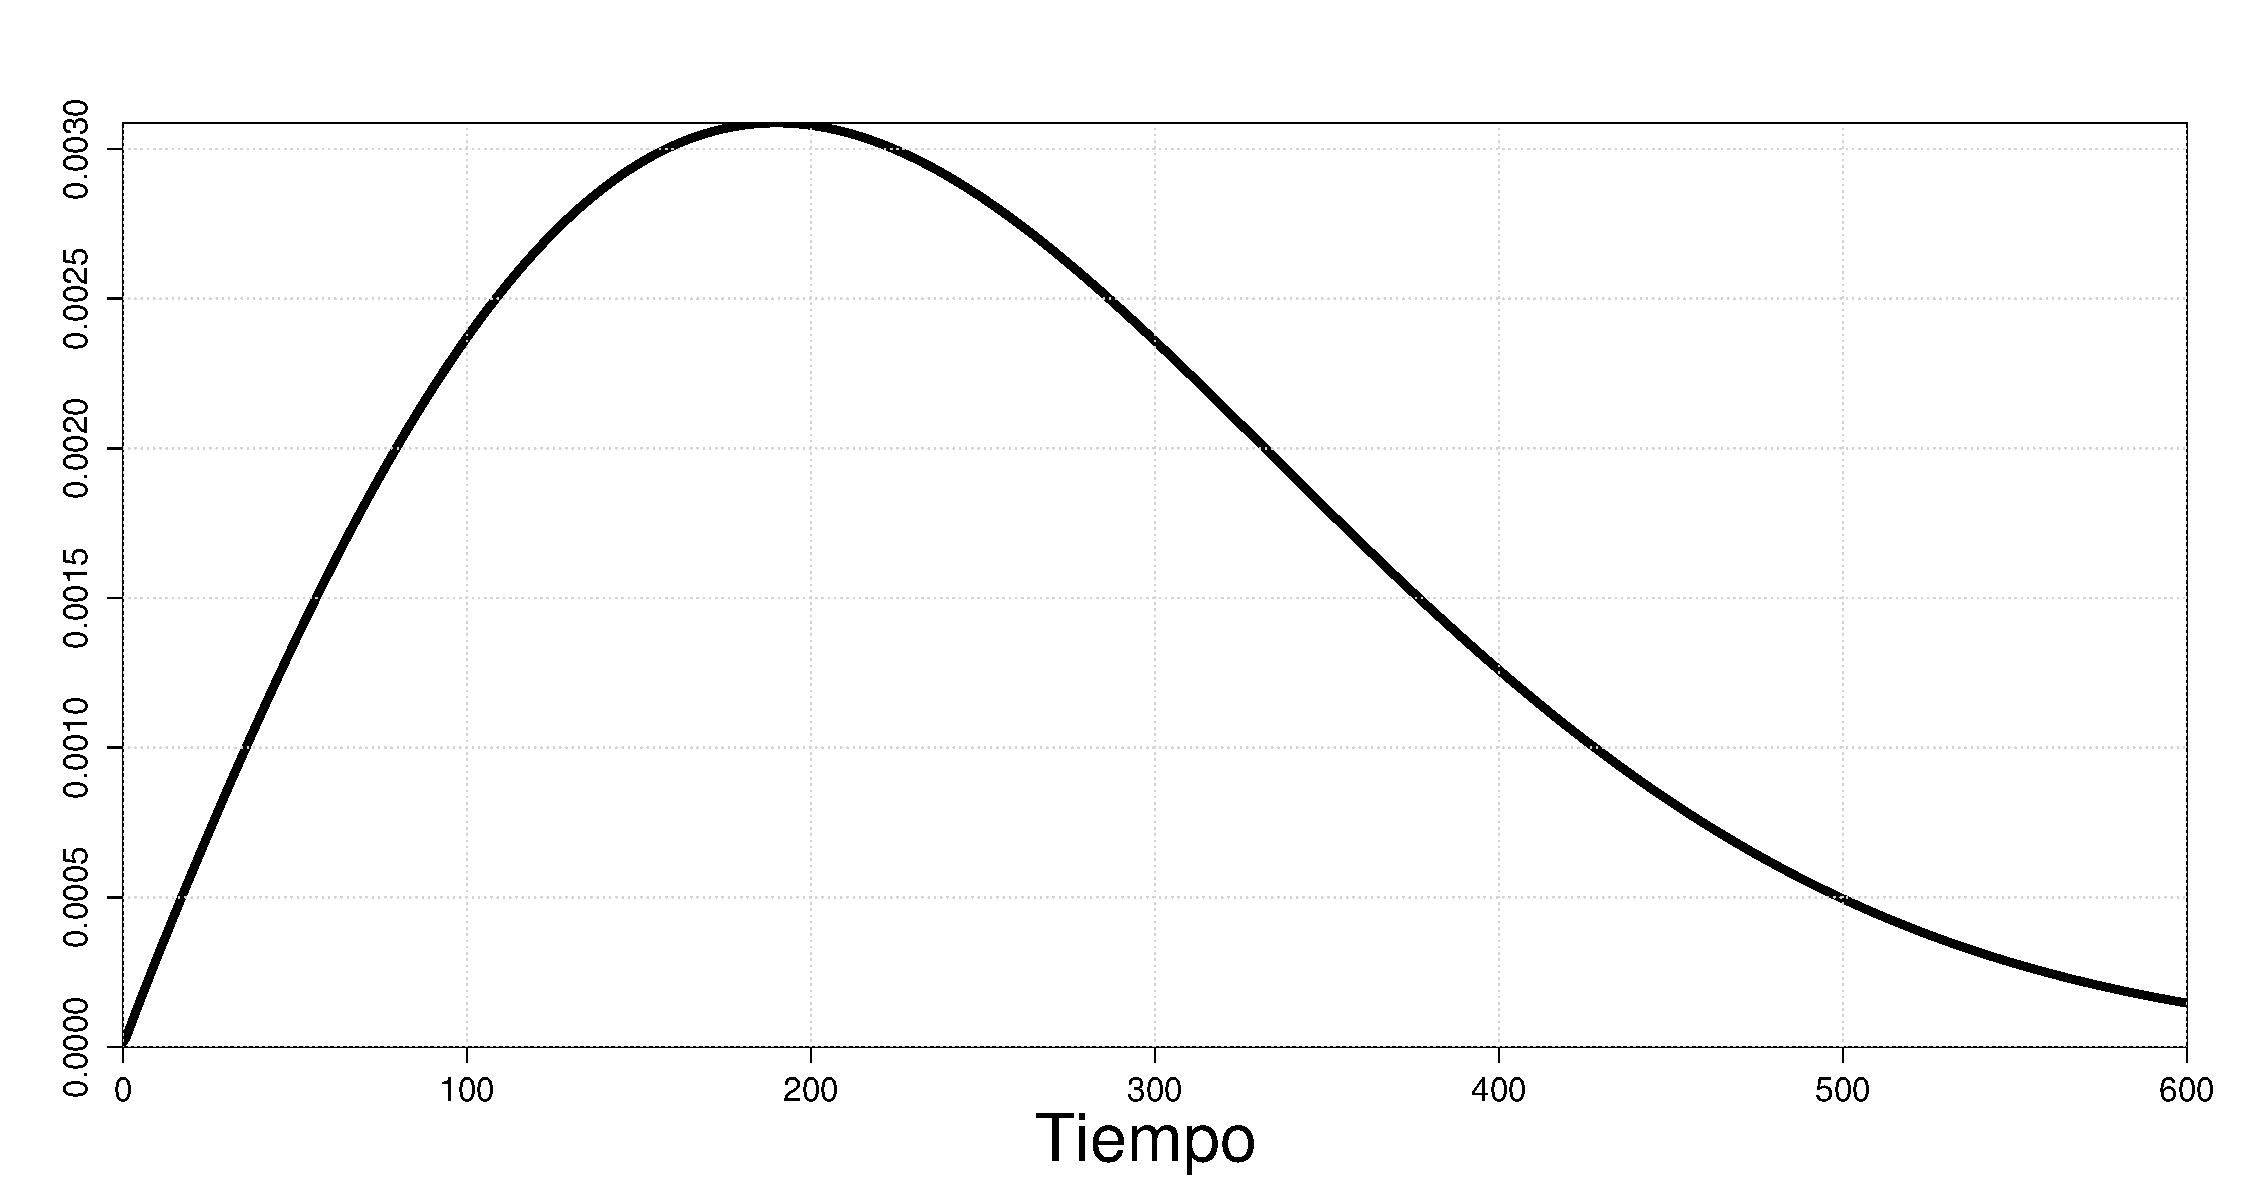
\includegraphics[scale=0.2]{app.pdf}
\vspace{-0.5cm}\caption{{\bf Funci\'on de densidad a priori.}\label{risk1}}
\end{figure}


\begin{figure}
\centering
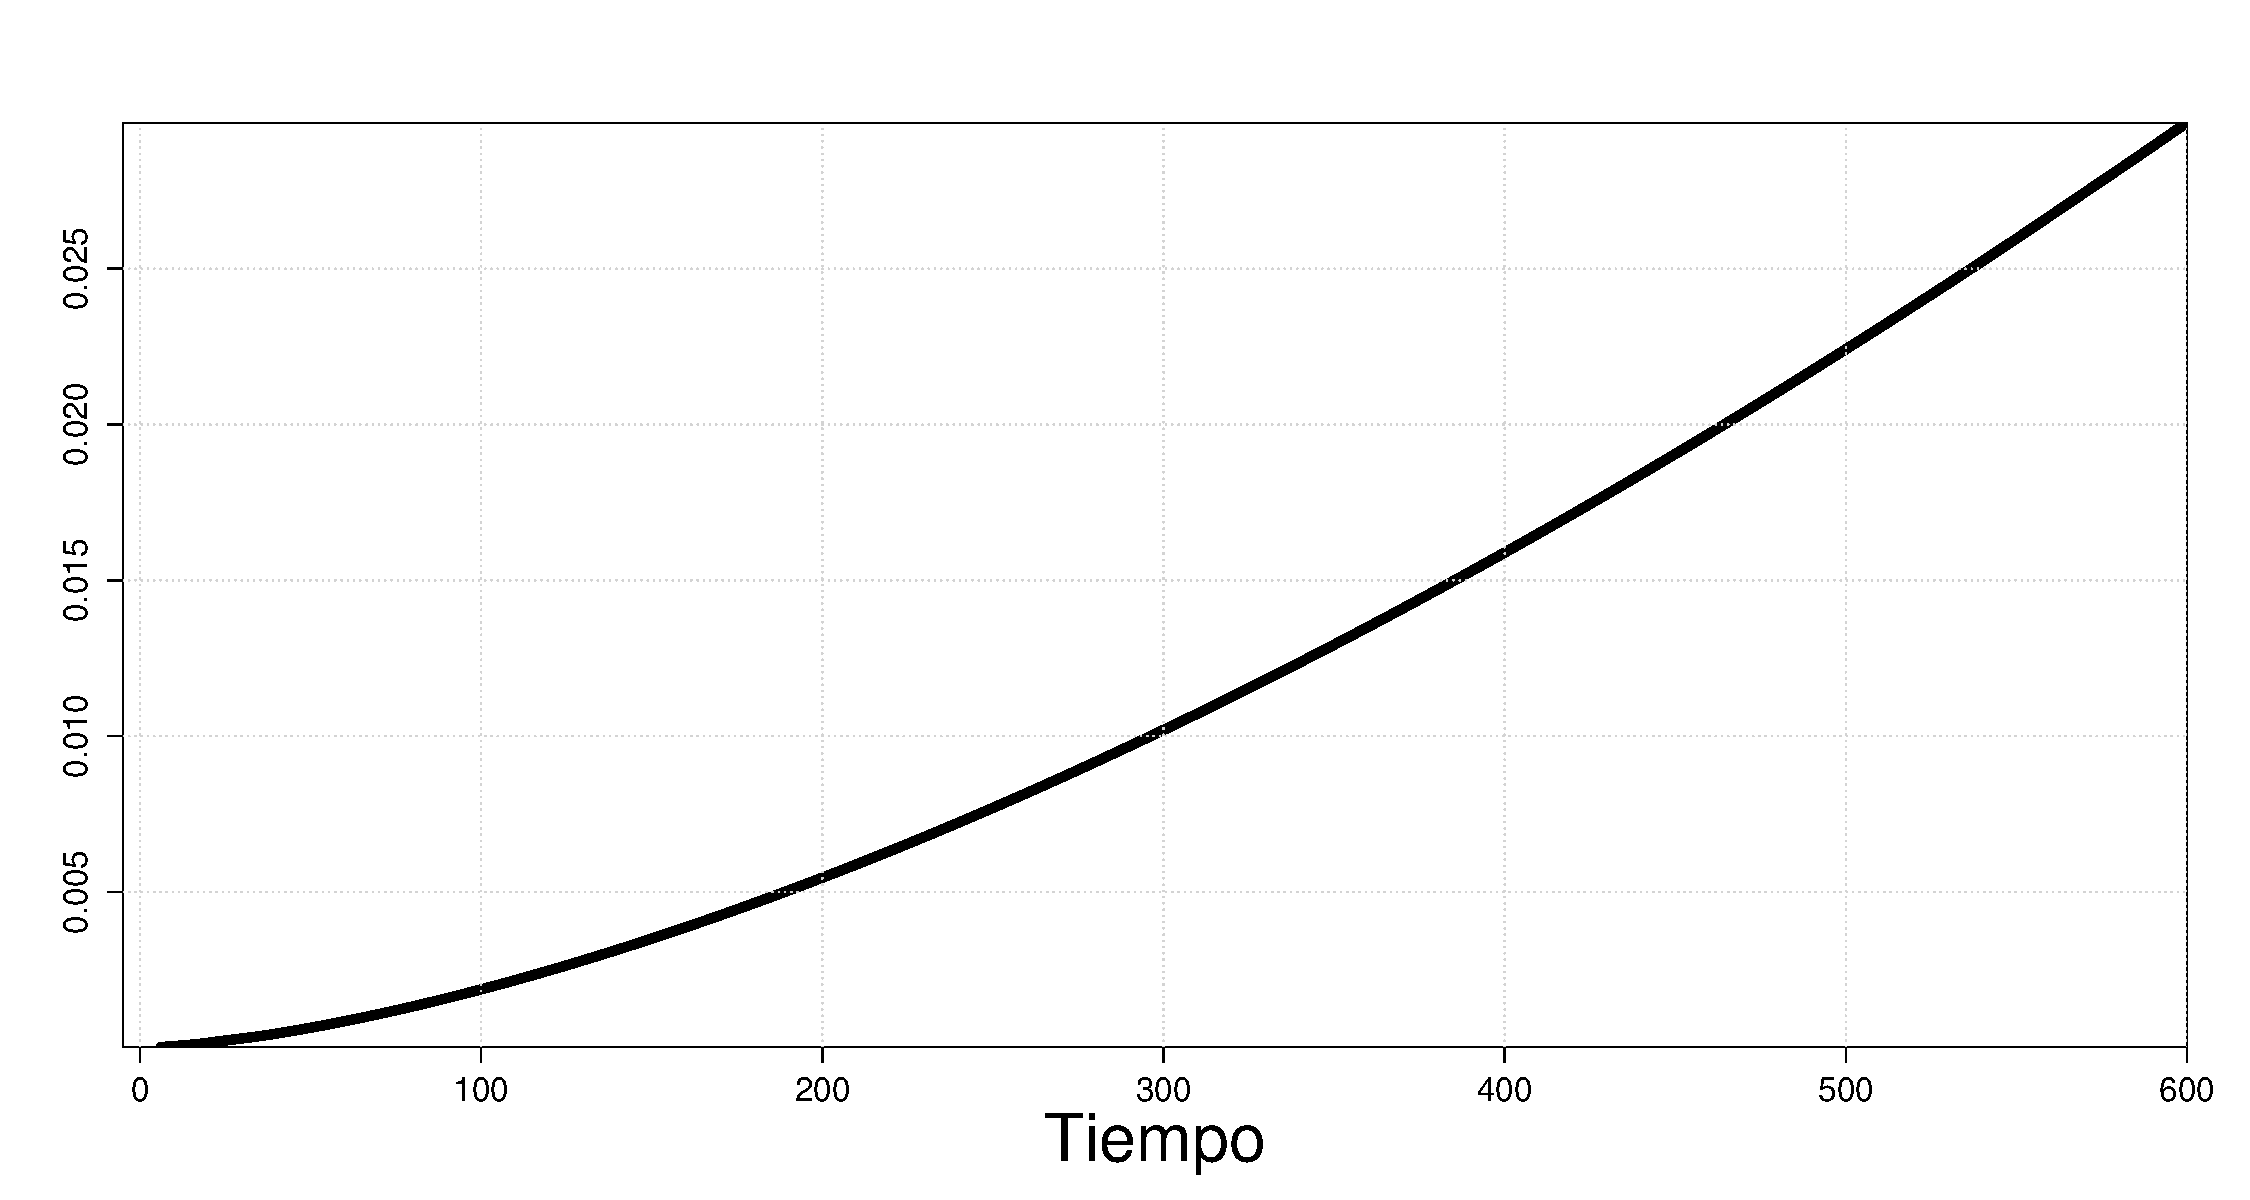
\includegraphics[scale=0.2]{r2meses.pdf}
\vspace{-0.5cm}\caption{{\bf Funci\'on de riesgo a priori.}\label{risk2}}
\end{figure}

\section{Distribuci\'on  Posterior}
\noindent Recordando que  $T$ es la variable aleatoria que representa los tiempo de vida de los transformadores, su funci\'on de verosimilitud esta dada por (\ref{tiempos}) y las distribuciones (\ref{beta}), (\ref{eta}). 
La distribuci\'on posterior es 

\begin{eqnarray*}
f(\beta,\eta|T)&\propto&\mbox{Verosimilitud} \times \mbox{A priori} \\
&=& f(T|\beta,\eta)f(\beta,\eta)
\end{eqnarray*}
Suponiendo que existe independencia a priori, entre los par\'ametros $\beta$ y $\eta$ se tiene:

\begin{eqnarray}\label{pos}
f(\beta,\eta|T)&=&f(T|\beta,\eta)f(\beta,\eta)\\\nonumber
&=& f(T|\beta,\eta)f(\beta)f(\eta)\\\nonumber
&=& \prod_{e_i=0}\frac{\beta}{\eta}\left(\frac{t_i}{\eta}\right)^{\beta-1}\exp \left\{-\left(\frac{t_i}{\eta}\right)^{\beta}\right\}\prod_{e_i=1}\exp\left\{-\left(\frac{t_i}{\eta}\right)^{\beta}\right\}\\\nonumber
& &\frac{1}{b^a\Gamma(a)}\beta^{a-1}\exp\left\{-\frac{\beta}{b}\right\}\frac{1}{b_1^{a_1}\Gamma(a_1)}\eta^{a_1-1}\exp\left\{-\frac{\eta}{b_1}\right\}
\end{eqnarray}

\noindent La Ecuaci\'on (\ref{pos}) muestra que la distribuci\'on posterior de los par\'ametros, es una expresi\'on compleja y no f\'acil de evaluar.  En tales situaciones se recurre a la ayuda de m\'etodos computacionalmente intensivos que permiten simular una muestra de la distribuci\'on posterior, tales como algoritmos MCMC, que son ampliamente
utilizados en estas situaciones.

\begin{figure}[h]
\begin{minipage}[b]{0.5\linewidth}
 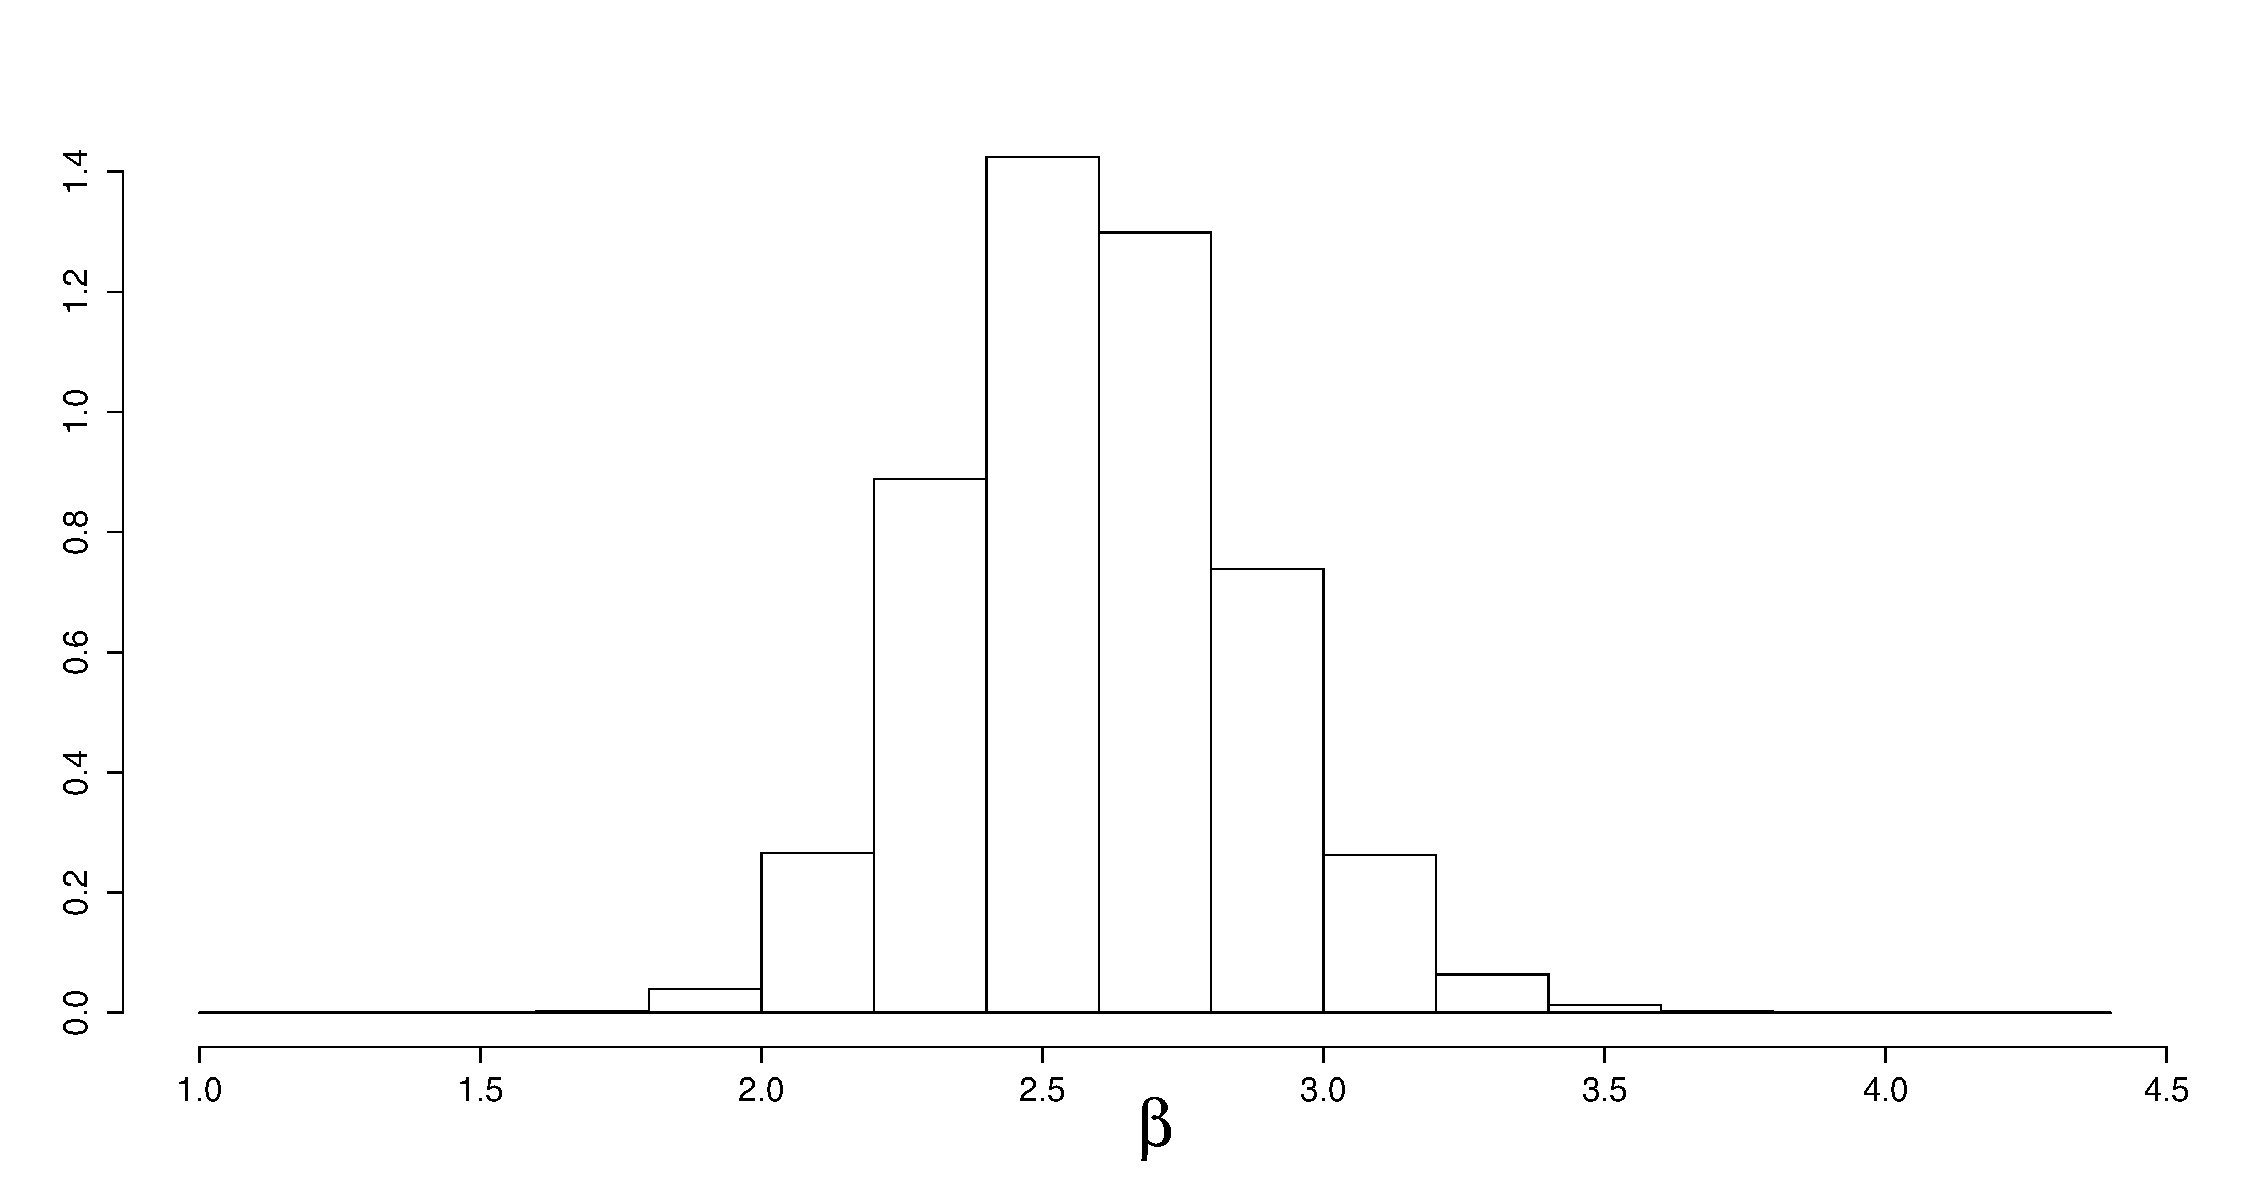
\includegraphics[scale=0.2]{pos1.pdf}
  \caption{{\small \bf Salida t-walk para $\beta.$}}
  \label{his1}
\end{minipage}
\begin{minipage}[b]{0.45\linewidth}
  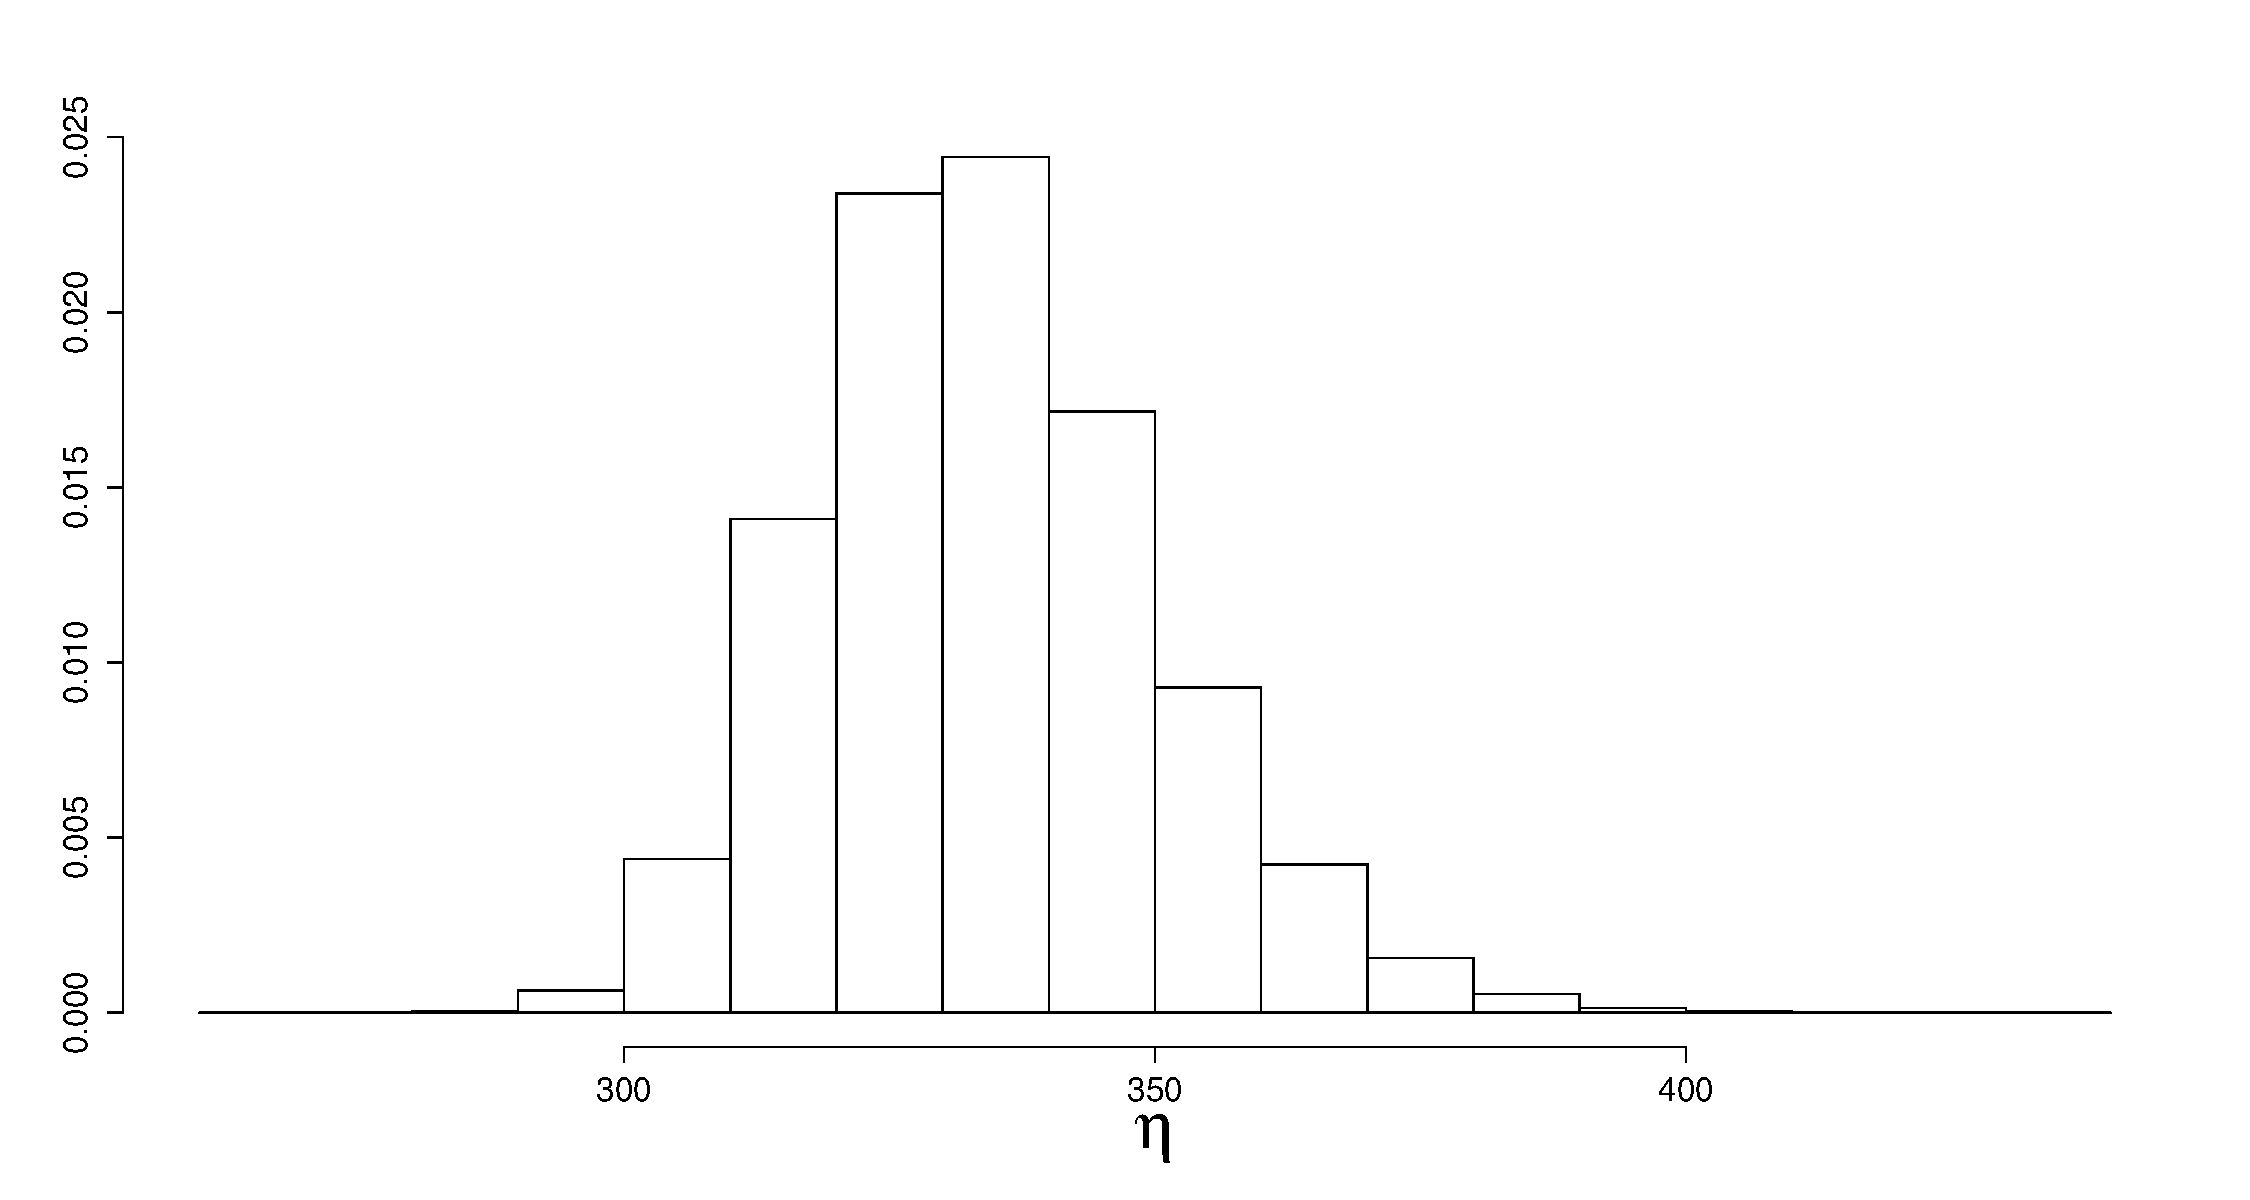
\includegraphics[scale=0.2]{pos2.pdf}
  \caption{{\small \bf Salida t-walk para $\eta.$}}
  \label{his2}
\end{minipage}
\end{figure}

\noindent Para conocer la muestra de la distribuci\'on posterior se uso el lenguaje de programaci\'on R, y la funci\'on t-walk que permite obtener tal muestra [{\bf \ref{r}}]. Con la funci\'on t-walk se realizaron $900,000$ iteraciones para obtener la muestra deseada (\ref{pos}). Los resultados est\'an resumidos en las Figuras \ref{his1} y \ref{his2} que indican los valores en los que  se concentran $\beta$ y $\eta$. Por ejemplo en la Figura 
 \ref{his1} los valores de $\beta$ m\'as probables oscilan alrededor de 2.5, pero puede tomar valores de 2 hasta 3.5. Mientras que en la Figura \ref{his2} observamos los valores para $\eta$ que presentan un rango de entre 280 y 400. Siendo alrededor de 335 el m\'as probable.
 
 \begin{figure}
\begin{center}
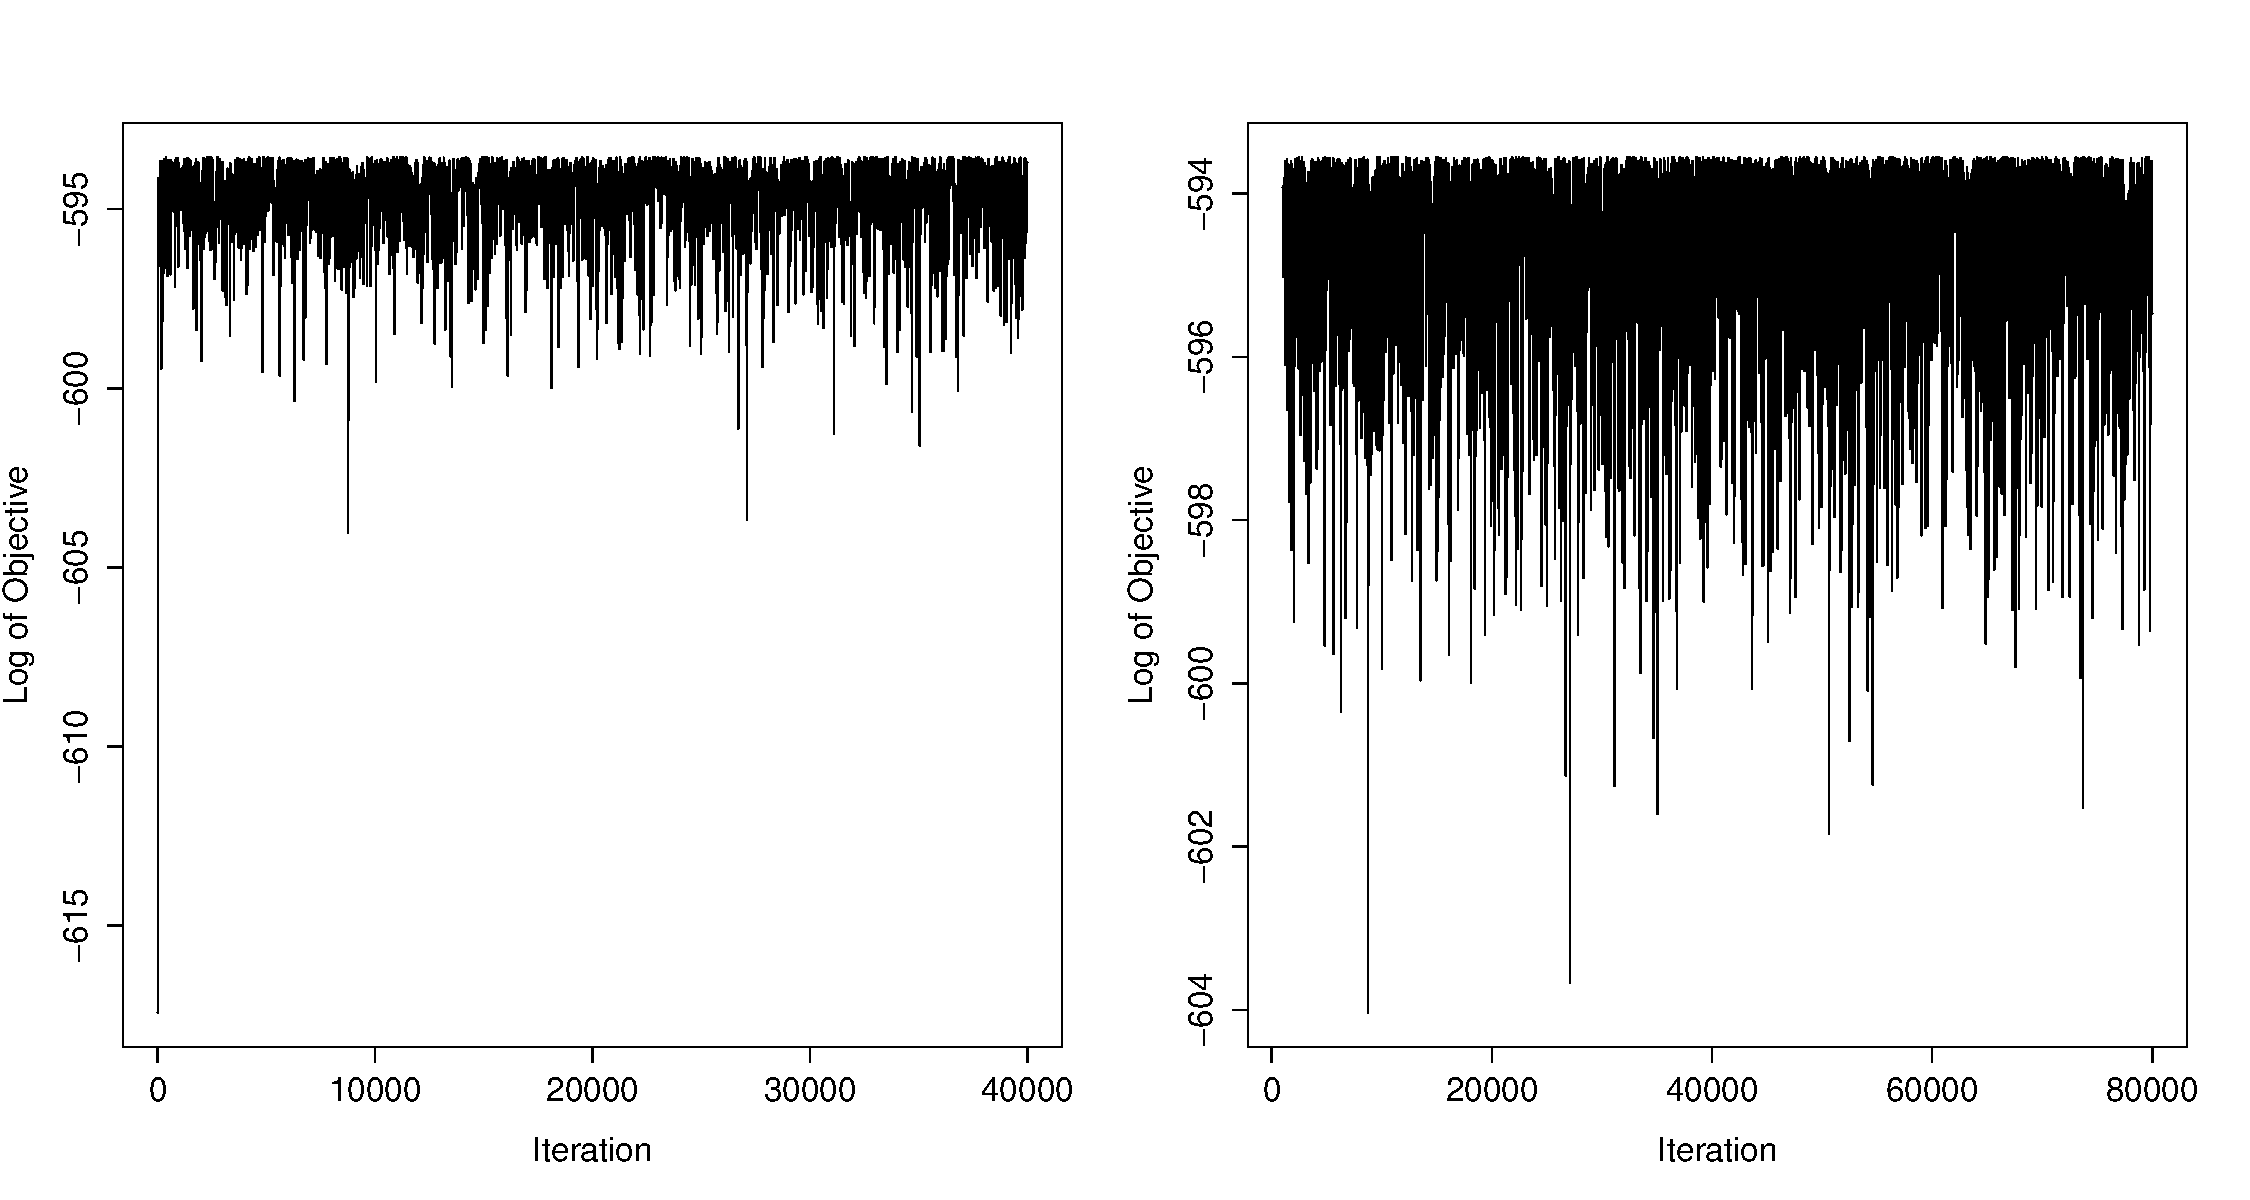
\includegraphics[scale=0.3]{logObj1.pdf} %logobj1
\end{center}
\vspace{-1cm} \caption{{\bf Dentro de t-Walk, se suele emplear, la funci\'on logaritmo de la distribuci\'on objetivo para evaluar la convergencia del m\'etodo. La gr\'afica muestra el comportamiento de esta funci\'on.}\label{mlog}}
\end{figure}

\begin{figure}
\begin{center}
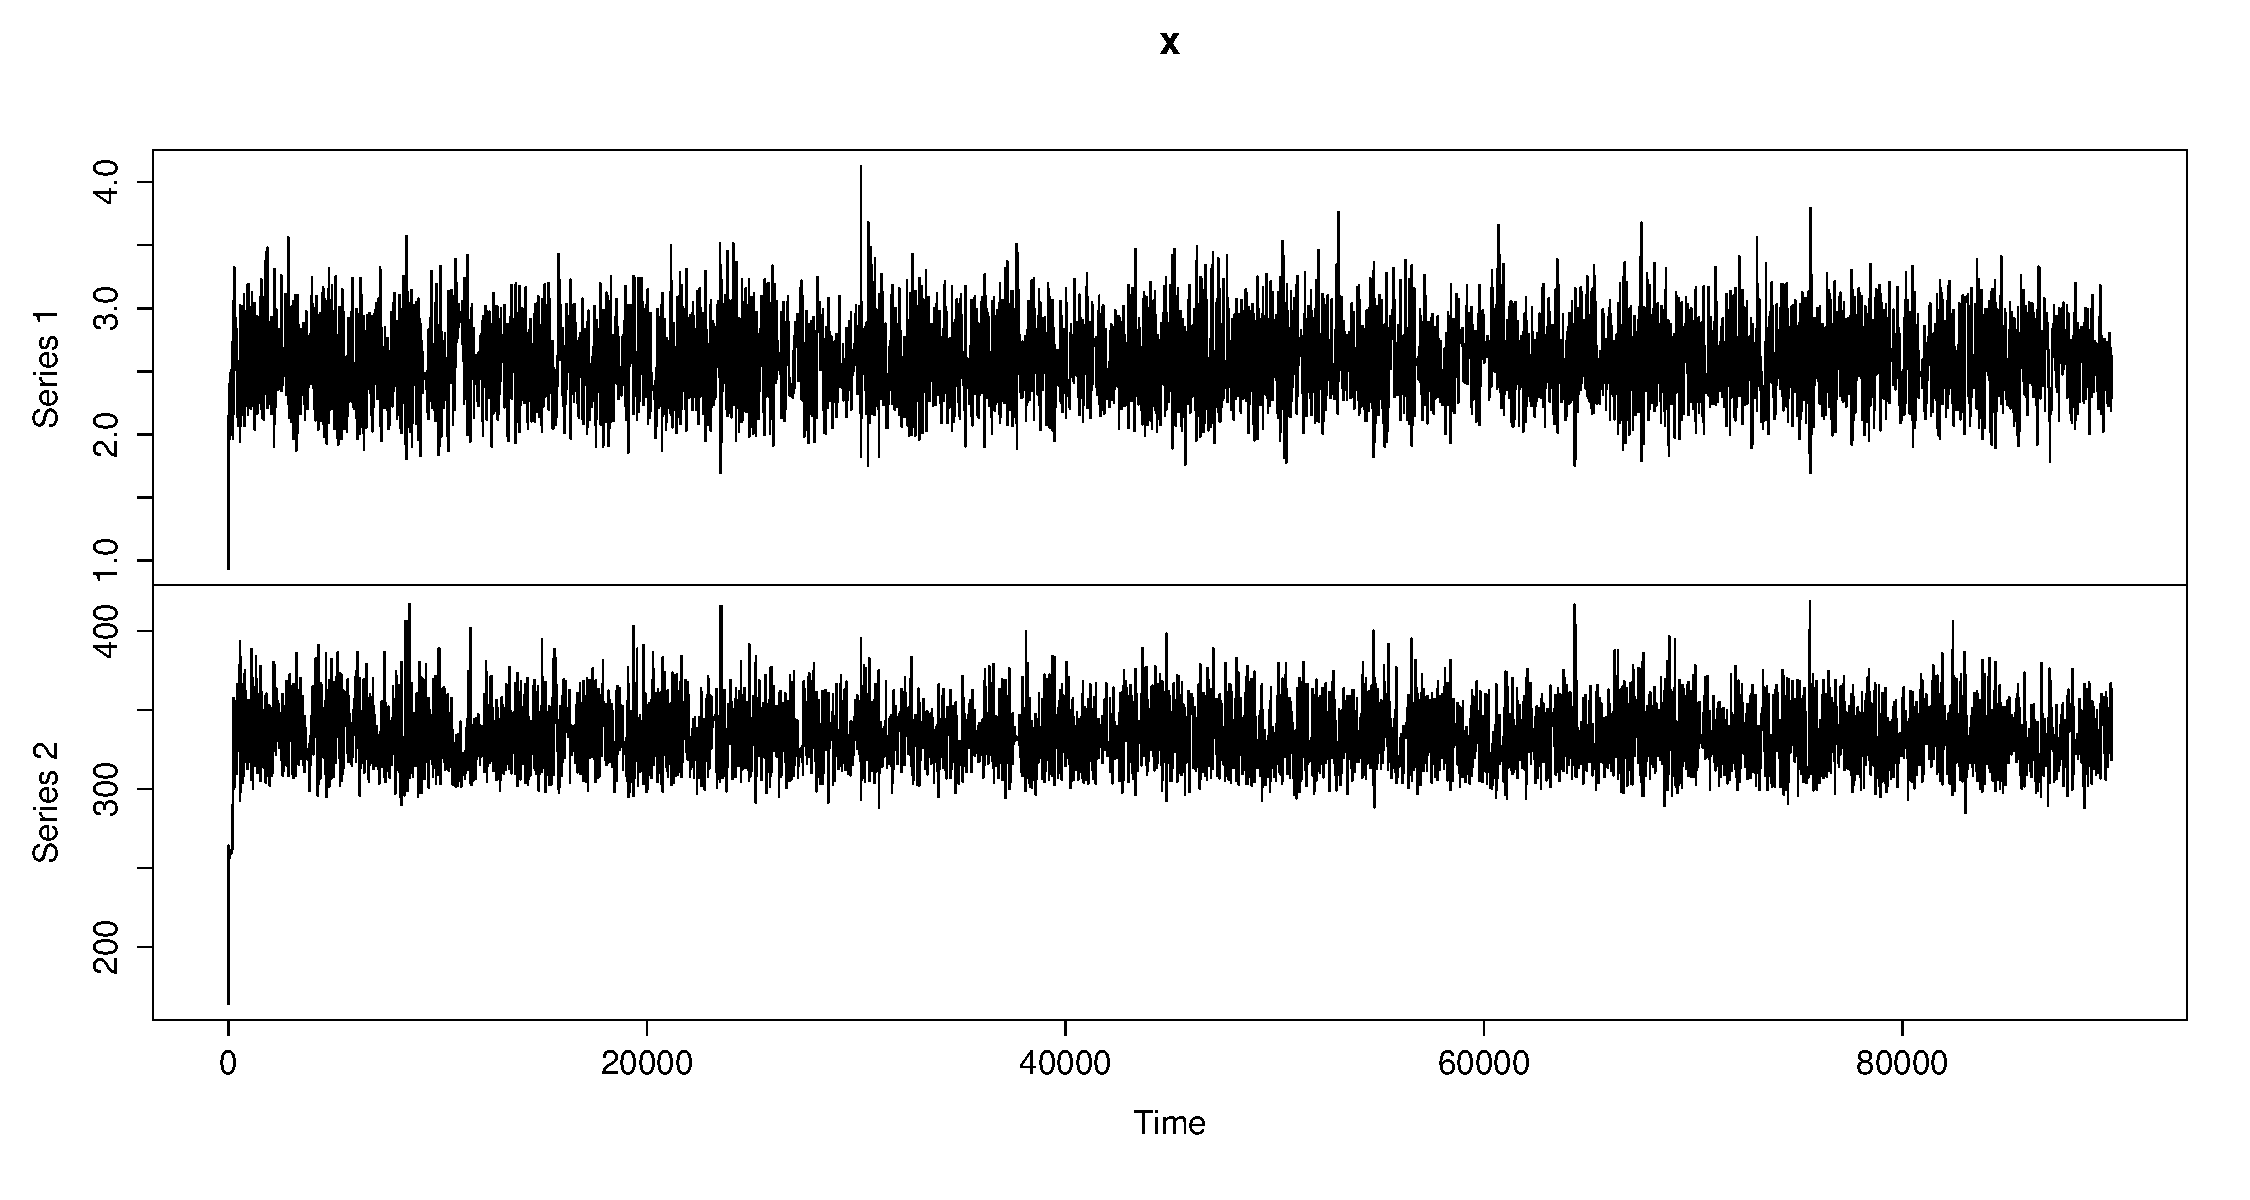
\includegraphics[scale=0.25]{serie.pdf}
\end{center}
\vspace{-1cm}\caption{{\bf Series de convergencia de los par\'ametros $\beta$ y $\eta$, proporcionados por la funci\'on t-Walk. La serie 1 corresponde a $\beta$ y la serie 2 a $\eta$.}\label{serie}}
\end{figure}

%\begin{figure}
%\begin{center}
%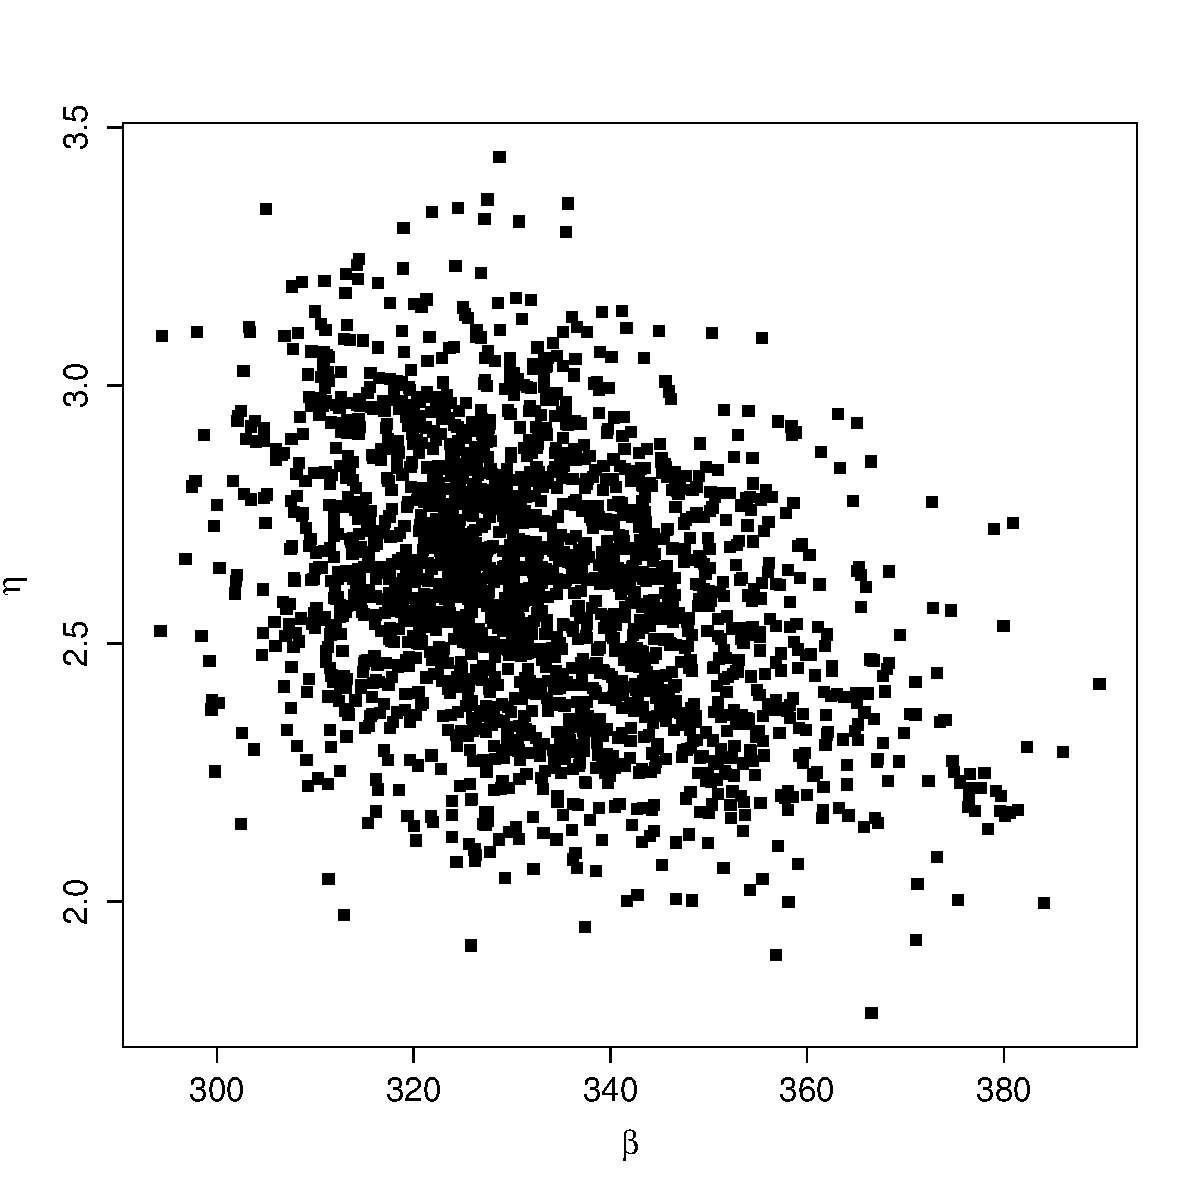
\includegraphics[scale=0.4]{corre1.pdf}
%\end{center}
%\vspace{-1cm}
%\caption{{\bf Muestra MCMC obtenida de la funci\'on t-Walk, graficada puntualmente con los valores de $\beta$ y $\eta$.}}
%\label{serie}
%\end{figure}

\noindent Las Figuras \ref{mlog} y \ref{serie}, muestran el an\'alisis de convergencia obtenido empleando la funci\'on t-walk. Observamos que la convergencia se da en un n\'umero de iteraciones relativamente peque\~no.\\[0.2cm]
\noindent Con la muestra, se obtiene  la densidad predictiva posterior, que describe el comportamiento de los tiempos de vida de los transformadores. La Figura \ref{apripos} muestra esta distribuci\'on, considerando la incertidumbre de los par\'ametros desconocidos $\beta$ y $\eta$.
\begin{figure}
\begin{center}
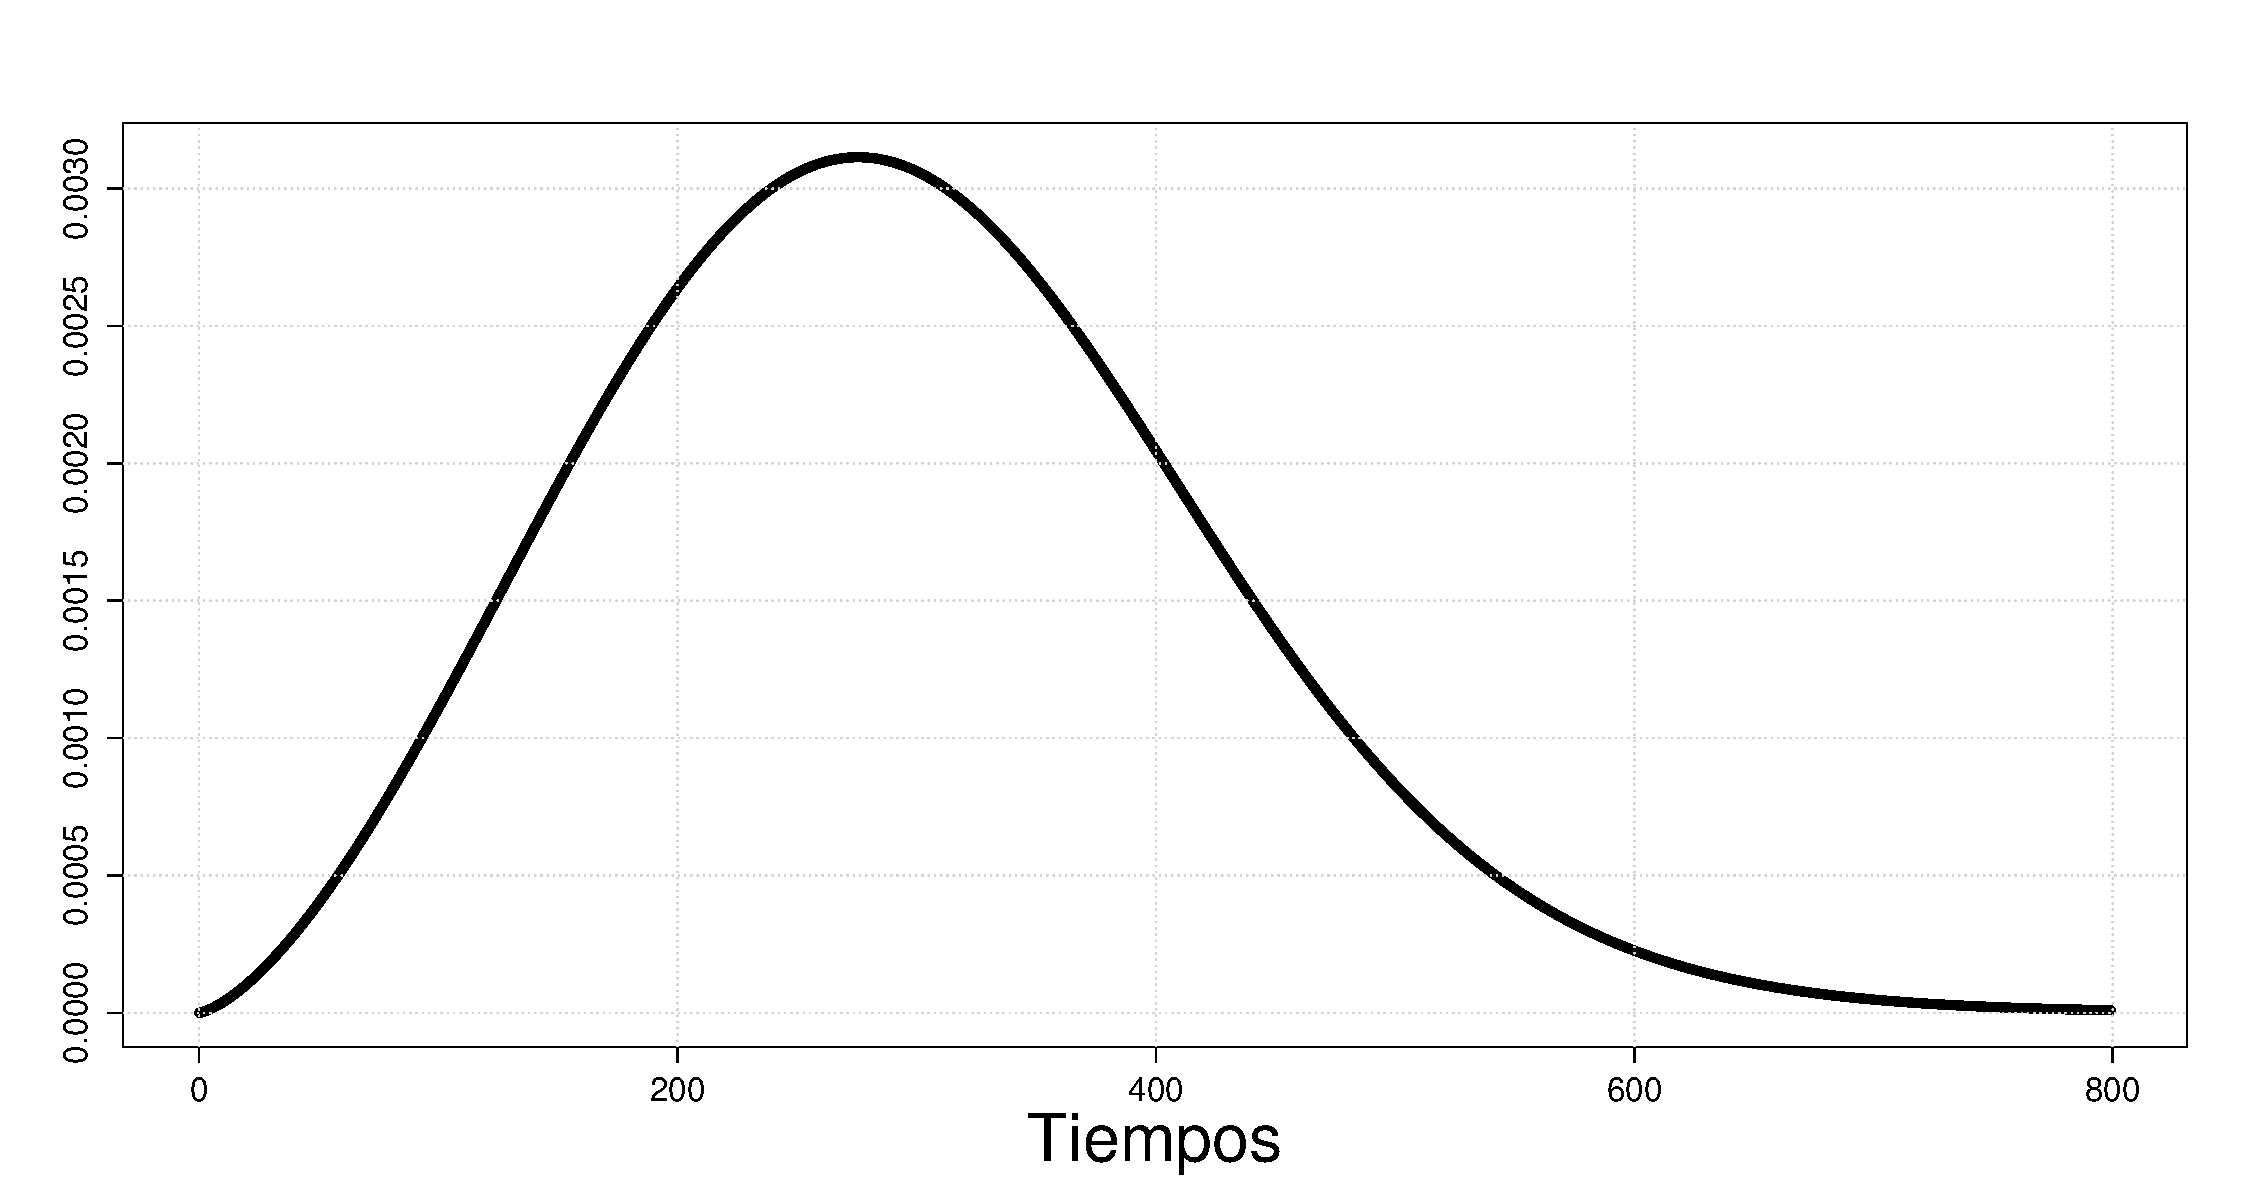
\includegraphics[scale=0.25]{DenPos.pdf}
\end{center}
\vspace{-1 cm} \caption{{\bf Densidad predictiva  posterior.}\label{apripos}}
\end{figure}


\noindent La funci\'on de confiabilidad y la funci\'on de riesgo se presentan en las Figuras \ref{CPos} y \ref{RPos} respectivamente. La confiabilidad decae lentamente. Se espera que a los 200 meses la probabilidad de que un transformador no falle es de 0.8. En la Tabla  \ref{conf} se muestran las probabilidades  de la funci\'on de confiabilidad, de los transformadores que segu\'ian operando despu\'es del 2006.

\begin{table}[h!]\small
\centering
\caption{\bf Confiabilidad de los transformadores que segu\'ian funcionando despu\'es del 2006.}\label{conf}
\vspace{.2cm}
\begin{tabular}{c|cccccc}
\toprule[0.6mm]
Meses de trabajo &8 &  20 & 32  & 56 & 80 &116  \\
\hline
Confiabilidad & 0.99 &0.99     &  0.99   &0.98 &0.97  &0.93 \\
\hline
Meses de trabajo &152 &164 &176& 188& 272& 296  \\
\hline
Confiabilidad & 0.87  &0.85   &  0.82     & 0.79 &0.55  &0.47 \\
\toprule[0.6mm]
\end{tabular}
\end{table}

\begin{figure}
\begin{center}
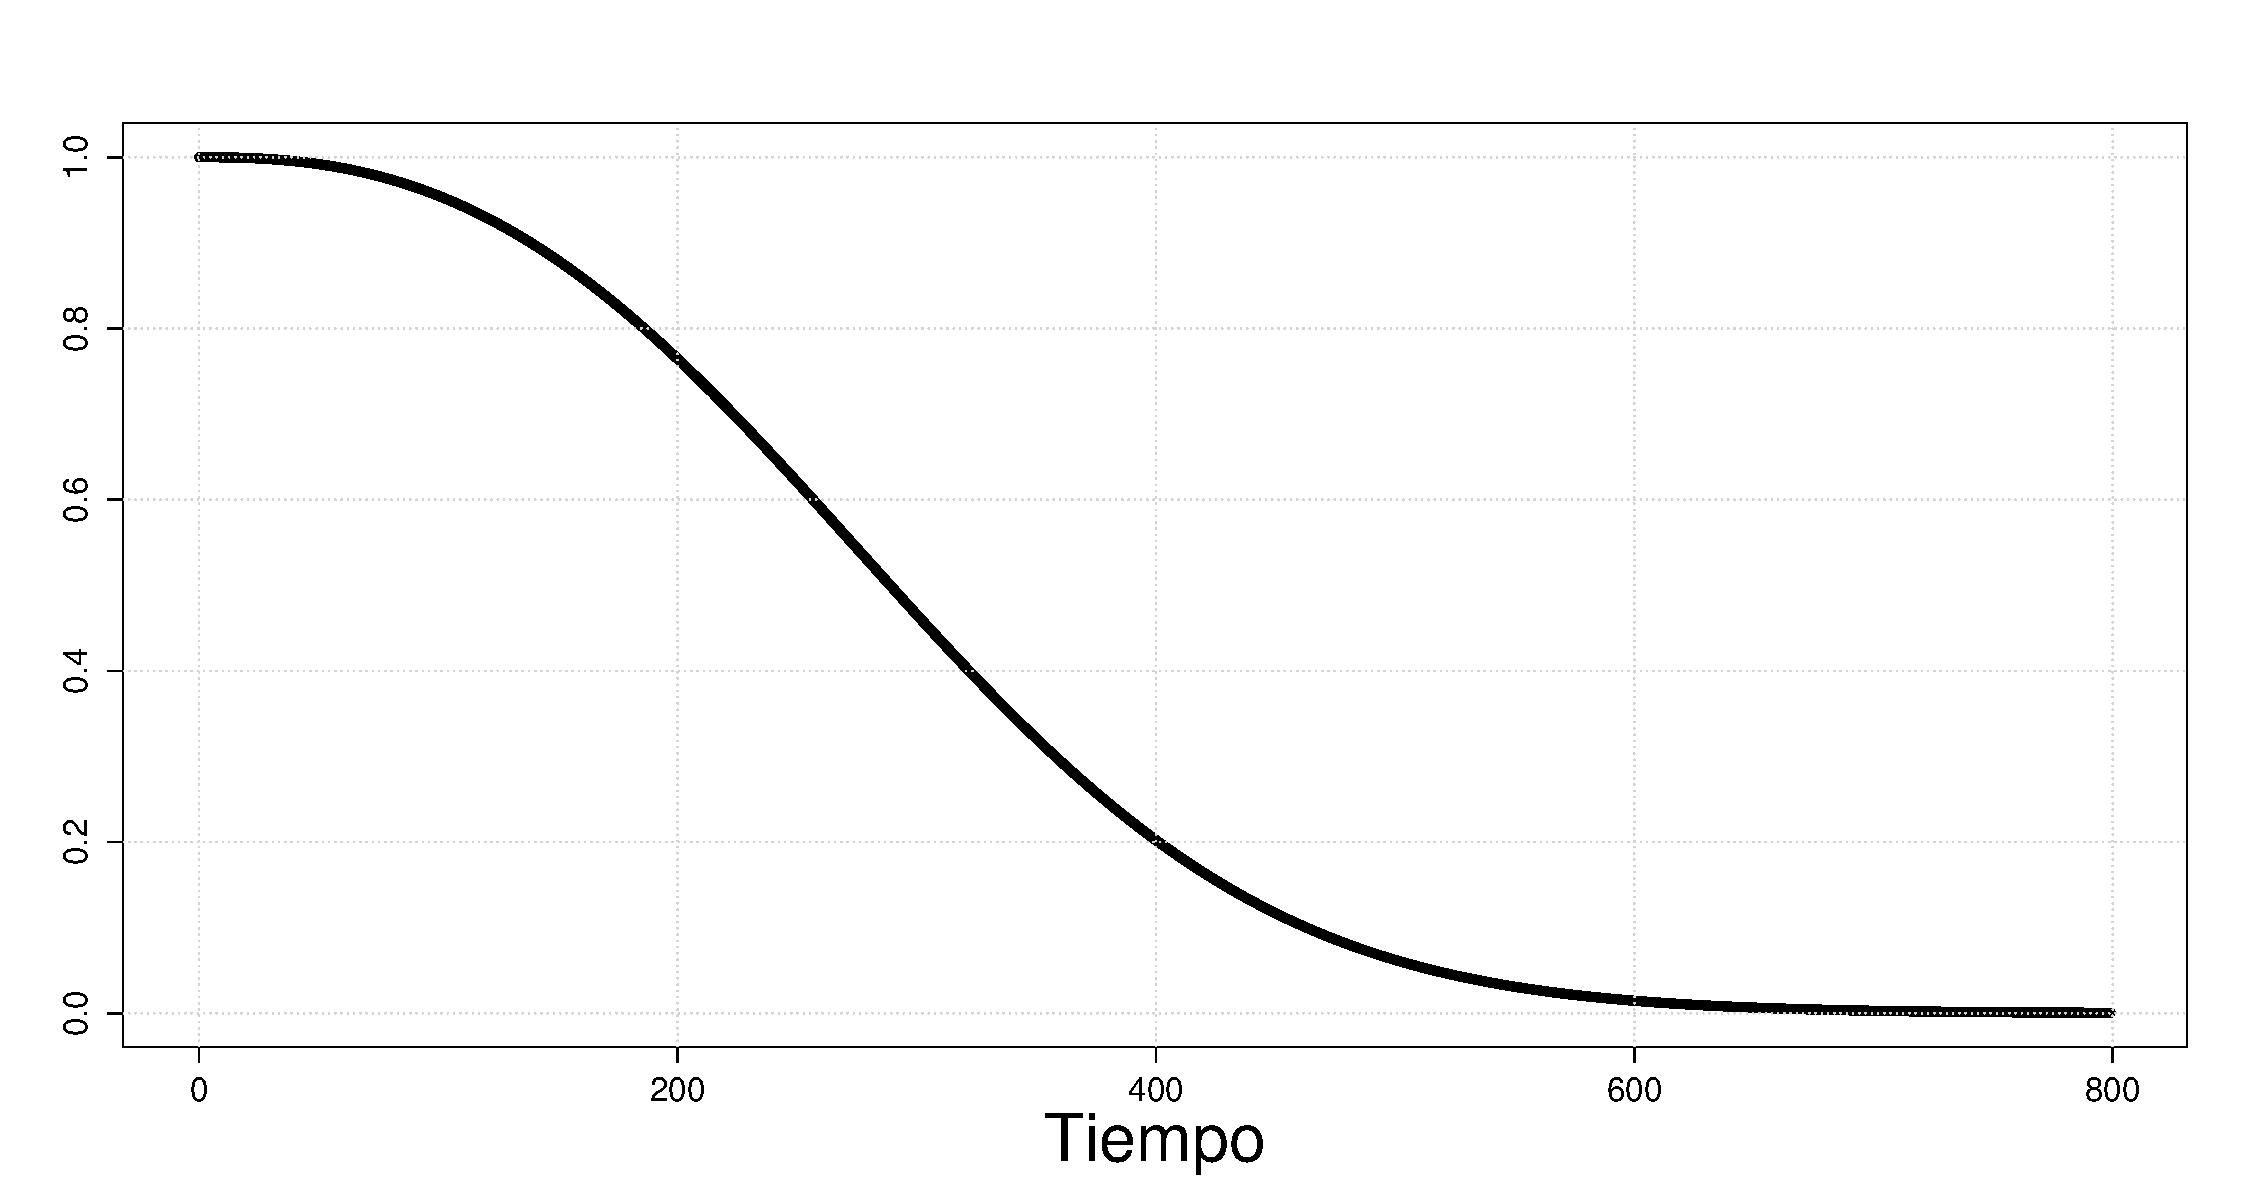
\includegraphics[scale=0.25]{ConPos.pdf}
\end{center}
\vspace{-0.5 cm} \caption{{\bf Confiabilidad posterior obtenida.}\label{CPos}}
\end{figure}


\noindent La probabilidad de que un transformador siga funcionando despu\'es de 8 meses es alta, de 0.99. Mientras que la probabilidad de que funcione  despu\'es de 12 a\~nos empieza a  decrecer, es de 0.87.\\
\noindent Un aspecto importante a evaluar es conocer la confiabilidad condicional, dada por: 
\vspace{-.1cm}
\begin{eqnarray*}
C(t_0|t)=P(T>t_0+t|T>t).
\end{eqnarray*}
\noindent  Esta indica la confiabilidad de un componente que ya ha vivido hasta un tiempo $t$. En la  Tabla \ref{ccc} se muestra la confiabilidad condicional de los transformadores que han vivido hasta un tiempo dado. 
\noindent Cuando el transformador ha trabajado 8 meses, la probabilidad de que siga funcionando un a\~no m\'as, es practicamente 1 y la probabilidad de que trabaje 12 a\~nos m\'as es 0.96, indicando que es un componente nuevo y su tiempo de vida es bueno, a\'un despu\'es de 12 a\~nos de operaci\'on. Por otra parte cuando un transformador ya ha vivido 308 meses (25 a\~nos), la probabilidad de que opere un a\~no m\'as es 0.4 y la probabilidad que viva 20 a\~nos m\'as es casi cero.

\begin{table}[ht]\small
\begin{center}
\caption{\bf Confiabilidad condicional de los transformadores que segu\'ian en funcionamiento despu\'es del 2006}\label{ccc}
\vspace{.3cm}
\begin{tabular}{c|c|c|c|c|c}
\toprule[0.6mm]
 Meses de trabajo ($t$) & C(1 a\~no$|t$) &C(2 a\~nos$|t$ ) &C( 7  a\~nos $|t$) & C(12 a\~nos$|t$) & C(20 a\~nos$|t$) \\ 
\toprule[0.6mm]
%\hline
  8& 1.00 & 1.00 & 0.99 & 0.98 & 0.96 \\ 
  20 & 1.00 & 1.00 & 0.98 & 0.96 & 0.91 \\ 
  32 & 0.99 & 0.99 & 0.96 & 0.93 & 0.85 \\ 
  56 & 0.98 & 0.98 & 0.92 & 0.86 & 0.73 \\ 
  80 & 0.96 & 0.95 & 0.88 & 0.78 & 0.62 \\ 
  116 & 0.92 & 0.90 & 0.79 & 0.66 & 0.47 \\ 
  152 & 0.85 & 0.83 & 0.68 & 0.54 & 0.34 \\ 
  164 & 0.82 & 0.80 & 0.65 & 0.50 & 0.30 \\ 
  176 & 0.80 & 0.77 & 0.61 & 0.46 & 0.26 \\ 
  188 & 0.76 & 0.73 & 0.57 & 0.42 & 0.23 \\ 
  272 & 0.52 & 0.48 & 0.31 & 0.19 & 0.08 \\ 
  296 & 0.44 & 0.41 & 0.25 & 0.15 & 0.06 \\ 
  308 & 0.41 & 0.37 & 0.23 & 0.13 & 0.05 \\ 
\bottomrule[0.6mm]
\end{tabular}\label{condicional}
\end{center}
\end{table}

\noindent Para obtener  los valores de la Tabla \ref{condicional}, se considera la incertidumbre de los par\'ametros desconocidos $\beta$ y $\eta$, la cu\'al se refleja por los valores obtenidos de la muestra de la distribuci\'on posterior, dada en (\ref{pos}), siendo que de (\ref{a}) y (\ref{b}), 
\begin{eqnarray*}
C(t_0|t)=\int P(T>t_0+t|T>t,\beta,\eta)f(\beta,\eta)d\beta d\eta.
\end{eqnarray*}

\noindent Dicha integral es aproximada con la muestra de la distribuci\'on generada mediante el empleo del algoritmo MCMC (t-Walk) por medio de la expresi\'on (\ref{b}). 
\noindent Para evaluar el patr\'on de desgaste de la unidades en la Figura \ref{RPos} observamos la funci\'on de riesgo de los transformadores, esta crece de manera lenta.
\begin{figure}[h!]
\begin{center}
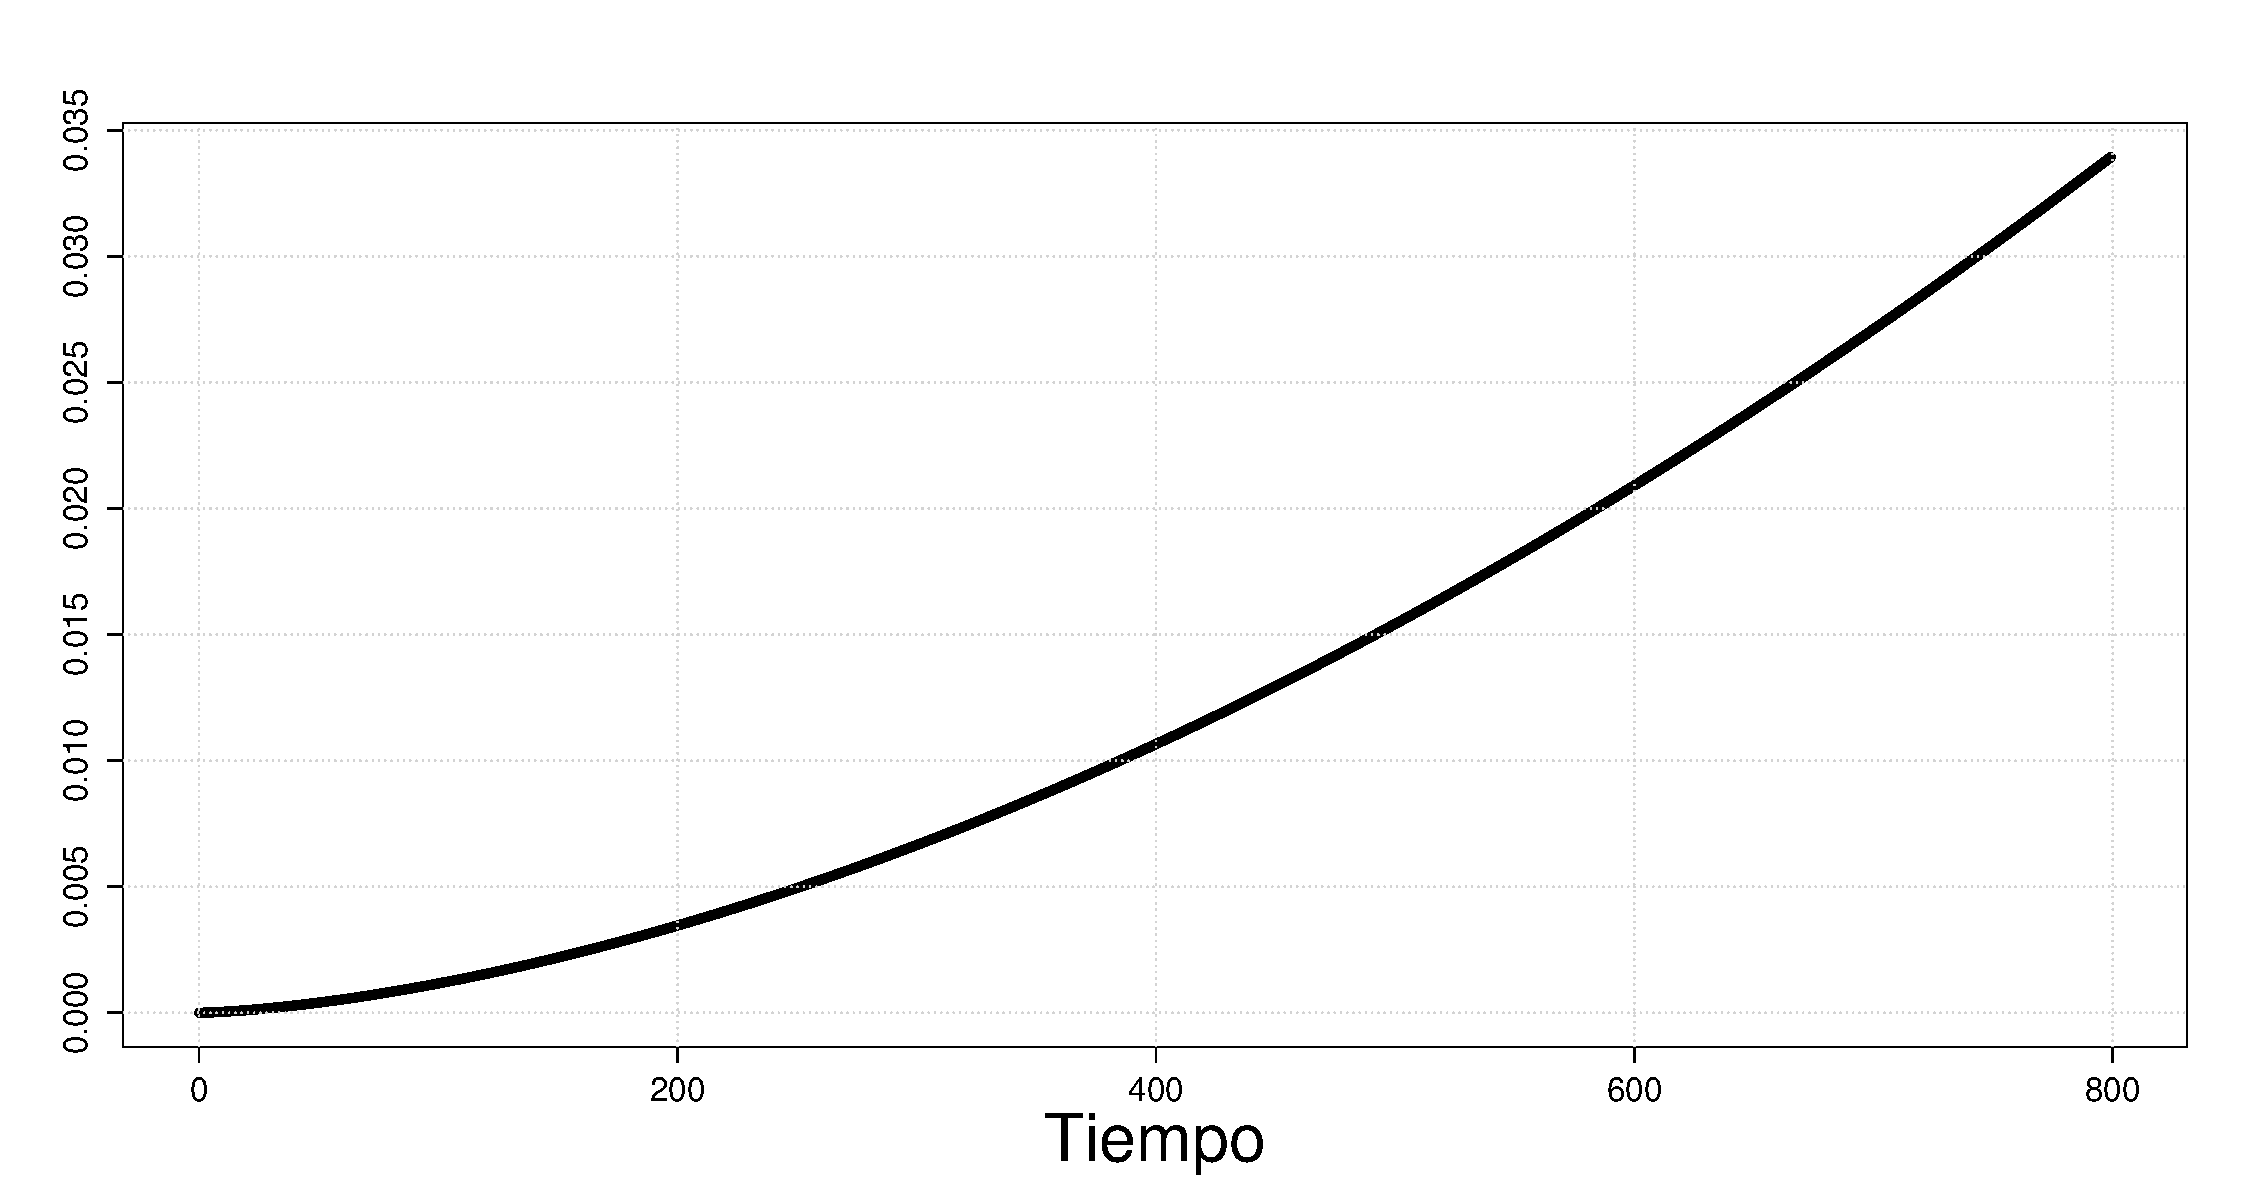
\includegraphics[scale=.25]{Rpos.pdf}
\end{center}
\vspace{-1 cm}{\caption{\bf  Tasa de falla mensual, empleando la muestra de la funci\'on t-Walk.}\label{RPos}}
\end{figure}
\noindent Por lo tanto cabe recalcar que las gr\'aficas de las Figuras \ref{apripos}, \ref{CPos} y \ref{RPos} son aproximaciones empleando la muestra de la distribuci\'on posterior obtenida y aplicando (\ref{b}).



%\end{document}
\newpage \thispagestyle{empty} \cleardoublepage